\begin{figure}[t]
\centering
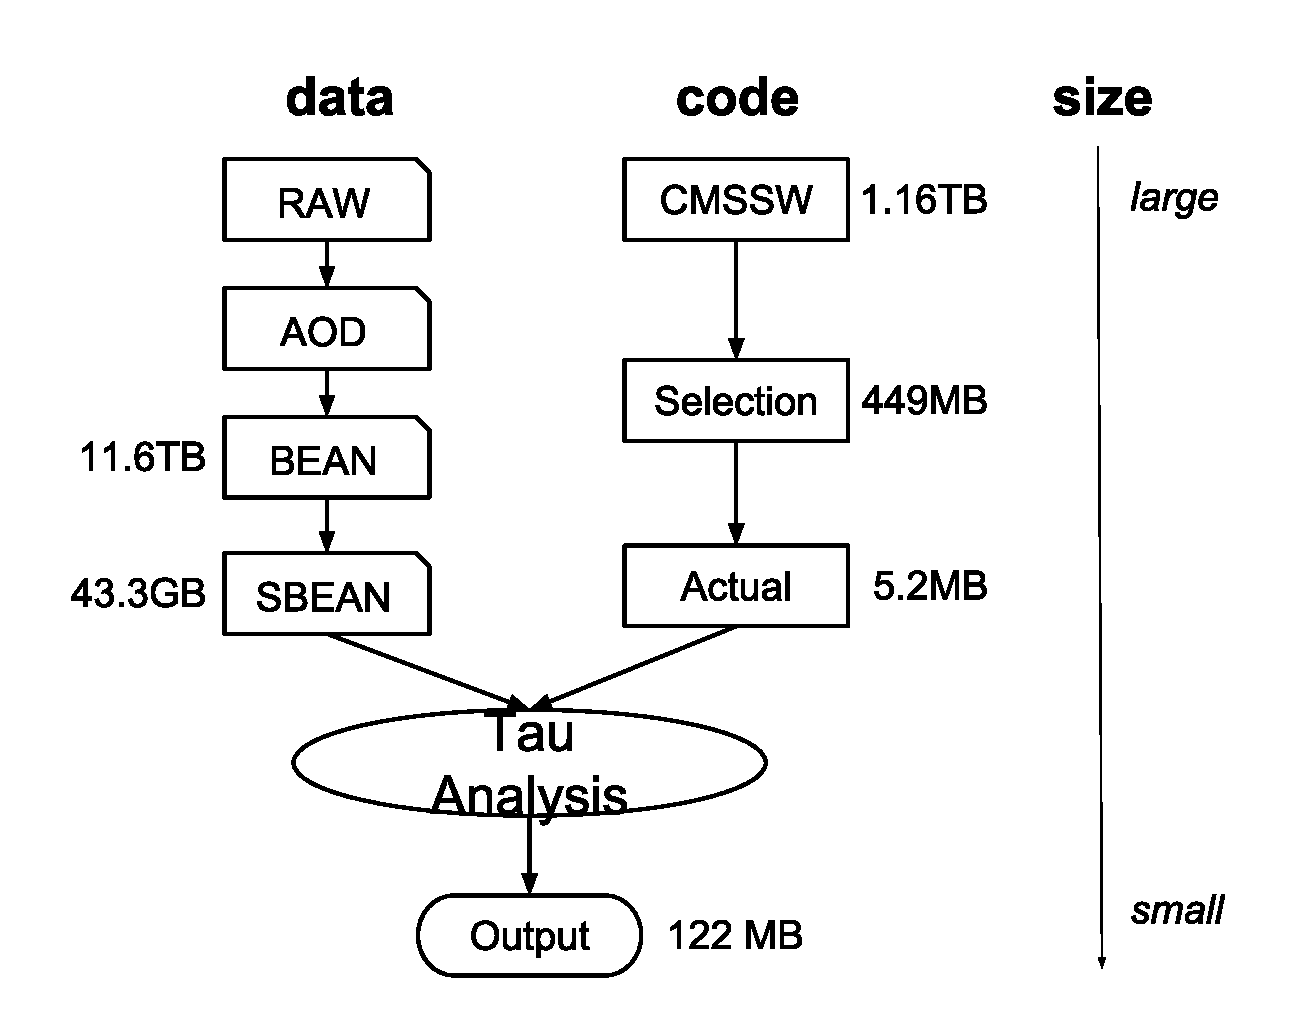
\includegraphics[width=.5\textwidth]{data-code-size.eps}
\caption{Inputs to Tau Roast}
\label{fig:data-code-size}
\end{figure}

\section{Overview of Tau Roast}

The application which is the study of this paper is an CMS application~\cite{collaboration2008cms} called \emph{TauRoast}.
It searches for cases where the Higgs boson decays to two tau leptons~\cite{chatrchyan2013search}.
Since the tau leptons are very short-lived, they are not observed directly, but by the particle decay products 
that they generate.  So, the analysis must search for detector
events that show a signature of decay products compatible with both hadronic tau and top decays.  

Figure~\ref{fig:data-code-size} shows that both the code and data
that form \emph{TauRoast} are drawn from large repositories through
multiple steps of reduction.  A preservation strategy must weigh
whether to store the large repositories completely, the fragments
used by an artifact, or something in between.

{\bf Code Sources.} Like many scientific codes, the central algorithm
of \emph{TauRoast} is expressed in a relatively small amount of
custom code developed by the primary author.  But, the code cannot
run at all without making use of an enormous collection of software
dependencies.  
The largest of these repositories is the CMS Software Distribution (CMSSW)~\cite{cms2006cms},
which contains many different tools, libraries, and utilities.  No single code uses anywhere close to all of these.  But, because it is widely used within the experimental researchers, it is common for users to simply expect that a particular version of the entire repository is available.
 
{\bf Data Sources.}
The CMS collaboration provides end-users with a pre-processed
and reduced data format, AOD~\cite{holtman2001cms}, 
which is based on the RAW output of the CMS detector readout electronics and reconstructed world-wide.
As AOD data are too large to be iteratively processed repetitively in
a physics analysis workflow, it is normally reduced further in
structural complexity and content.  For the analysis under
investigation here, this is a two-step process.  First, the AOD data
are processed at the Notre Dame working group cluster to BEAN (Boson Exploration Analysis Ntuple) events,
containing only trivial data containers packed in vectors.  This step
is time and CPU intensive and its output contains data of 11.6$\,$TB to be
analyzed by the tau analysis.
In the second step, the data are reduced to the ``Ntuple'' format,
which contains only events matching basic quality criteria and
fields relevant to \emph{TauRoast}.
Once the data has been reduced to Ntuples, TauRoast can be run as a single
process, and contains a stringent event selection to look only at high
quality candidate events for the underlying physical process.
Quantities from the relevant events can be
both plotted and used in multivariate analysis to determine the level
of expected signal in real data.

